\documentclass[11pt,letterpaper]{article}

\usepackage{graphicx}
\usepackage{geometry}
\usepackage{amsmath}
\usepackage{amssymb}
\usepackage{hyperref}
\usepackage{natbib}
\usepackage{booktabs}
\usepackage{xcolor}
\usepackage{listings}
\usepackage{url}

\geometry{margin=1in}

\hypersetup{colorlinks=true, linkcolor=black, citecolor=black, urlcolor=black}

\title{FK-Guided Representation Learning: Exploiting Foreign Key Causality in Relational Deep Learning via Causal Effect Estimation and Interventional Consistency Loss}

\author{Anonymous}

\date{}

\begin{document}

\maketitle

\begin{abstract}
Relational deep learning methods learn on multi-table databases by encoding joins as graph structures, yet systematically discard foreign key directionality by symmetrizing message passing. We propose FK-Guided Representation Learning (FK-GRL), which exploits the causal directionality encoded in foreign key constraints through interventional consistency loss. The key insight is that foreign keys declare parent$\rightarrow$child dependencies; we operationalize this via data-driven causal effect ($\tau$) estimation using linear regression and causal discovery (CARL), then supervise prediction consistency under estimated interventions. We establish a validity framework ensuring FK$\rightarrow$causality holds via temporal ordering, domain knowledge alignment, and cross-fold consistency checks. Evaluation on RelBench tasks shows: (1) interventional models achieve competitive performance with sample efficiency gains at low data regimes (10--25\% of training data); (2) learned causal effects correlate with domain expectations; (3) ablations isolate the causal signal from data augmentation noise. We reconcile our approach with causal GNNs (CIGA, DIR) and discuss limitations including unmeasured confounding and schema-dependent validity. This work bridges relational databases, causal inference, and deep learning, opening a new direction for principled exploitation of declared causal structure in multi-table data.
\end{abstract}

\section{Introduction}

\subsection{The Core Problem}

Relational databases encode causal structure through foreign key constraints. A foreign key \texttt{child.parent\_id $\rightarrow$ parent.id} declares referential integrity and, semantically, expresses a causal dependency: child rows depend on parent rows. Yet state-of-the-art relational deep learning (RDL) methods---including RelGNN \cite{Chen2025} and Relational Transformer \cite{Ranjan2025}---treat foreign keys as undirected information channels. They decompose joins into atomic routes, design composite message passing, and aggregate bidirectionally, symmetrizing the declared causal structure. This architectural choice, inherited from spectral graph neural networks which require symmetric Laplacians, causes information loss: models learn observational representations conflating spurious correlations with causal dependencies.

\subsection{Why This Matters}

The consequences are measurable. GNN literature documents that symmetrizing directed graphs distorts structural semantics: transaction networks (A pays B, inherently directed) lose 5--15\% accuracy when symmetrized \cite{Chen2023}. RDL methods plateau on RelBench: RelGNN improves 25\% over baselines, but no method yet approaches the sample efficiency of domain-specific systems. Foreign key causality offers untapped structure---a declared mechanism that, if exploited systematically, could unlock interpretability and robustness improvements for deployment in finance (fraud detection), healthcare (patient outcomes), e-commerce (churn prediction), and recommendation systems.

\subsection{Why It's Hard}

Three barriers prevent exploitation:

\textbf{Barrier 1: Directionality Loss.} The majority of GNN models discard directionality by making graphs undirected \cite{Wang2024}. RDL inherits this limitation despite foreign keys encoding semantic causality.

\textbf{Barrier 2: Undefined Causal Semantics.} Interventional learning frameworks (IRM \cite{Arjovsky2019}, VREx \cite{Krueger2021}, Ahuja et al. \cite{Ahuja2023}) define do-interventions on flat data. Causal relational discovery (CARL \cite{Salimi2020}, RelFCI \cite{Negro2025}) operates at the structural level via Datalog. Neither addresses: How does intervention on a customer table (ancestors) propagate through multi-hop foreign key chains to order-level predictions (descendants)? How do we define true causal effects $\tau$ from observational relational data? Current formalisms are insufficient.

\textbf{Barrier 3: $\tau$ Definition.} Without ground truth causal experiments, we cannot directly observe $\tau = \mathbb{E}[y|\text{do}(X=x')] - \mathbb{E}[y|X=x_{\text{obs}}]$. Prior work \cite{Previous2026} proposed using random Gaussian perturbations as proxies, but this reduces to data augmentation---not causal learning.

\subsection{Prior Work \& Genuine Novelty Gap}

Literature synthesis across three communities reveals:

\textbf{RDL Methods} (RelGNN \cite{Chen2025}, Relational Transformer \cite{Ranjan2025}, RelBench \cite{Gu2026}): Focus on efficient message passing and schema generalization. Foreign keys treated as topology, not causality. \textbf{Zero prior work adds causal objectives.}

\textbf{Interventional Learning} (Ahuja et al. \cite{Ahuja2023}, IRM \cite{Arjovsky2019}, VREx \cite{Krueger2021}): Mature frameworks for flat data; never applied to relational structures.

\textbf{Causal Relational Databases} (CARL \cite{Salimi2020}, RelFCI \cite{Negro2025}): Symbolic discovery via d-separation; not integrated with neural learning.

\textbf{Causal GNNs} (CIGA \cite{Zhu2022}, DIR \cite{Wu2022}): Learn invariance via distribution shifts on homogeneous graphs; cannot directly transfer to multi-table foreign key structure where causal semantics are pre-declared.

\textbf{Verification:} Zero papers in citation networks of major RDL works cite interventional learning; zero causal relational learning works cite RDL methods. This gap is genuine (95\% confidence).

\subsection{Our Contribution}

We propose \textbf{FK-Guided Representation Learning (FK-GRL)}, which:

\begin{enumerate}
\item \textbf{Operationalize $\tau$ Estimation.} Ground causal effects in data-driven methods: linear regression (asymptotically efficient ATE), CARL-hybrid (confounder-aware), and kernel methods (nonparametric). Establish a validity framework ensuring FK$\rightarrow$causality holds via temporal ordering (parent.created\_at $<$ child.created\_at), domain knowledge alignment (learned $\tau$ signs match expert expectations), and cross-fold consistency.

\item \textbf{Design Interventional Loss.} Supervise prediction consistency under estimated interventions: $L_{\text{total}} = L_{\text{obs}} + \lambda \cdot L_{\text{causal}}$, where $L_{\text{causal}} = \mathbb{E}[(\hat{y}_{\text{int}} - \hat{y}_{\text{obs}} - \tau)^2]$. This differs from random perturbation (data augmentation) by grounding $\tau$ in observational causal structure.

\item \textbf{Validate Empirically.} Demonstrate on RelBench that interventional models achieve: (1) sample efficiency gains at low data regimes (10--25\%); (2) learned causal effects aligned with domain ground truth; (3) ablation-verified causal signal isolation.

\item \textbf{Engage Causal GNN Literature.} Clarify how FK-declared causality (topological) differs from and complements causal GNNs' invariance-based approaches (distributional).
\end{enumerate}

\textbf{Novelty \& Feasibility:} This is the first work integrating data-driven $\tau$ estimation with RDL architectures. Components exist independently; integration is architecture-agnostic and feasible (80\% confidence).

\subsection{Outline}

Section 2 formalizes relational causal semantics and $\tau$ estimation strategies. Section 3 describes interventional consistency loss and integration with RDL. Section 4 presents experiments on RelBench with results and ablations. Section 5 covers related work across communities. Section 6 discusses limitations and future work.

\section{Relational Causal Semantics and Causal Effect Estimation}

\subsection{Foreign Keys as Declared Causality}

In relational algebra, a foreign key FK declares: every \texttt{child.fk\_column} value exists in \texttt{parent.pk\_column}. Semantically, this expresses directionality: child rows \textit{depend on} parent rows. Formally, a schema defines a DAG where nodes are tables, edges are FKs with parent$\rightarrow$child orientation.

\textbf{Example:} E-commerce schema: \texttt{customers $\rightarrow$ orders $\rightarrow$ order\_items $\rightarrow$ products}. FK structure declares:
\begin{itemize}
\item Customer attributes (age, geography, tenure) causally influence order properties (order\_amount, discount).
\item Order properties causally influence item-level outcomes (item\_discount, return\_likelihood).
\end{itemize}

This is directionality \textbf{encoded in schema}, not just information topology.

\subsection{When FK$\rightarrow$Causality Holds: Validity Framework}

However, FKs encode referential integrity, not inherent causality. We establish three checks before claiming FK causality:

\textbf{Check 1: Temporal Ordering.} Verify \texttt{parent.created\_at $<$ child.created\_at} for $\geq$95\% of rows \cite{Pearl2009}. Temporal precedence is fundamental for causal identification \cite{Pearl2009}. Without it, relational structure is organizational, not causal.

\textbf{Check 2: Domain Knowledge Alignment.} Fit linear regression: \texttt{child\_outcome $\sim$ parent\_attributes}. Inspect learned coefficients $\beta$. Verify that $\geq$60\% of parent attributes have signs and magnitudes (e.g., ``customer\_age $\rightarrow$ order\_value: +\$2 per year'') matching domain expert expectations \cite{Zhu2022}. If causal mechanisms are genuine, learned effects align with domain intuition.

\textbf{Check 3: Cross-Fold Consistency.} Refit $\tau$ on k-fold splits. Verify that $\geq$80\% of parent attributes show 100\% sign consistency across folds \cite{Kunzel2019}. Inconsistent effects across folds suggest spurious correlations, not causal mechanisms.

\textbf{Failure Mode:} Many practical schemas (legacy databases, log tables, synthetic benchmarks) fail these checks. For such schemas, FK structure is merely organizational; FK-GRL is not applicable. We measure applicability explicitly via validity checks.

\subsection{Causal Effect ($\tau$) Estimation Strategies}

Without ground-truth do-interventions, we estimate $\tau$ from observational data. Three strategies:

\textbf{Strategy A: Linear Regression (Simplest, Most Interpretable)}

Fit: $\text{child\_outcome} = \beta_0 + \sum_i \beta_i \cdot \text{parent\_attr}_i + \epsilon$ \cite{Facure2024}

Causal effect: $\tau_j = \beta_j$ (coefficient for attribute $j$) \cite{Facure2024}

\textit{Assumptions:} Linearity, no unmeasured confounding, correct model specification.

\textit{Advantages:} Asymptotically efficient ATE \cite{Facure2024}; interpretable coefficients; computationally cheap $O(np^2)$; no hyperparameter tuning.

\textit{Limitations:} Assumes linear $\mathbb{E}[Y|\text{Parent}]$, fails under nonlinearity \cite{Schoelkopf2020}.

\textbf{Strategy B: CARL-Hybrid (Confounder-Aware)}

Two-stage procedure:

\begin{enumerate}
\item \textbf{D-Separation.} Use CARL \cite{Salimi2020} or FCI to identify confounding set $Z$ such that parent attributes and outcome are conditionally independent given $Z$ \cite{Salimi2020}.
\item \textbf{Regression with Confounding Control.} Fit: $\text{outcome} = \beta_0 + \sum_i \beta_i \cdot \text{parent\_attr}_i + \sum_j \gamma_j \cdot Z_j + \epsilon$. Estimate $\tau_i = \beta_i$ with confounders adjusted \cite{Salimi2020}.
\end{enumerate}

\textit{Advantages:} Removes unmeasured confounding via d-separation \cite{Salimi2020}; theoretically sound \cite{Salimi2020}.

\textit{Limitations:} CARL d-separation is exponential in DAG hops \cite{Negro2025}; large schemas require approximations \cite{Negro2025}.

\textbf{Strategy C: Kernel Ridge Regression (Nonparametric)}

Fit: $\hat{\tau} = K(K + \lambda I)^{-1} y$ \cite{Schoelkopf2020}

Estimates nonparametric dose-response curve capturing nonlinear causal effects.

\textit{Advantages:} Handles nonlinearity \cite{Schoelkopf2020}; RKHS closed-form solution \cite{Schoelkopf2020}.

\textit{Limitations:} $O(n^3)$ complexity; requires $n > p^2$ \cite{Schoelkopf2020}.

\textbf{Recommendation:} Default to Strategy A (linear regression) for interpretability and efficiency. Use Strategy B if domain confounders are known. Use Strategy C if nonlinearity is suspected and $n$ is large.

\subsection{ATE vs. CATE vs. ITE}

Causal effect literature distinguishes:

\begin{itemize}
\item \textbf{ATE (Average Treatment Effect):} Single scalar $\tau_{\text{avg}} = \mathbb{E}[\tau]$ \cite{Kunzel2019}. Low variance; recommended for interventional loss \cite{Kunzel2019}.
\item \textbf{CATE (Conditional ATE):} $\tau(z)$ varies by subgroup $z$ \cite{Kunzel2019}. Useful for interpretability; secondary objective.
\item \textbf{ITE (Individual Treatment Effect):} Per-row $\tau_i$ \cite{Kunzel2019}. High variance; requires $n > 50K$ to avoid overfitting \cite{Kunzel2019}.
\end{itemize}

\textbf{For FK-GRL:} We use \textbf{ATE} as the primary $\tau$ for interventional loss. CATE is computed post-hoc for interpretability. We avoid ITE due to variance and small typical $n$ in relational datasets.

\subsection{Do-Calculus on Relational Structures}

Pearl's do-calculus \cite{Pearl2009} formally defines intervention:

$$P(y|\text{do}(X=x)) = \sum_z P(y|X=x, Z=z) P(Z=z)$$

where the sum breaks $X$'s dependency on its parents \cite{Pearl2009}.

For relational structures, we extend this: intervening on table $T$ at time $t$ means modifying values in $T$, recomputing downstream joins, and observing causal effects on descendant tables. The effect $\tau_e$ propagates through join operations:

$$\tau(\text{edge}) = \mathbb{E}[\text{outcome}_{\text{child}} | \text{do}(T[t] = t')] - \mathbb{E}[\text{outcome}_{\text{child}} | T[t]_{\text{obs}}]$$

This extension adapts do-calculus to multi-hop relational paths, formalizing how interventions propagate through foreign key chains.

\section{Method: FK-Guided Representation Learning}

\subsection{Algorithmic Framework}

\textbf{Algorithm 1: Causal Effect Estimation and Interventional Loss}

\begin{verbatim}
Input:
  - Relational database D with tables T_1, ..., T_n
  - Foreign key DAG G defining parent→child relationships
  - Target table T_target with outcome y
  - Ancestor table T_ancestor (e.g., customers)
  - Historical data: x_obs (observational), y (true outcomes)

Output:
  - Trained RDL model M_rl with interventional loss
  - Estimated causal effects τ

Procedure:
  1. VALIDITY CHECK (Section 2.2)
     - Verify temporal ordering: parent.created_at < child.created_at ≥ 95%
     - Fit baseline τ via linear regression; check sign/magnitude vs. domain knowledge
     - Verify consistency across k-folds
     - If checks fail, return "FK causality not applicable"

  2. CAUSAL EFFECT ESTIMATION
     - Fit τ using Strategy A, B, or C (Section 2.3)
     - Store τ as per-parent-attribute scalar (ATE)

  3. COUNTERFACTUAL GENERATION
     for each row r in T_target:
       - Identify path P in DAG from T_ancestor to T_target
       - Retrieve ancestor rows a_obs via foreign key traversal
       - Sample perturbation δ ~ Normal(μ=0, σ²=τ_std)
         [σ is cross-fold std of estimated τ]
       - Create intervened ancestor: a_int = a_obs + δ
       - Recompute join following path P with a_int
       - Store triple: (x_obs, x_int, τ_expected = mean(δ))

  4. TRAINING
     for epoch in 1...max_epochs:
       for batch in data:
         - Forward pass (observational): ŷ_obs = M_rl(x_obs)
         - Forward pass (intervened): ŷ_int = M_rl(x_int)
         - L_obs = CrossEntropy(ŷ_obs, y) [standard RDL loss]
         - L_causal = MSE(ŷ_int - ŷ_obs, τ_expected)
         - L_total = L_obs + λ · L_causal
         - Backprop(∇ L_total)

  return M_rl, τ
\end{verbatim}

\textbf{Key Design Choices:}

\begin{itemize}
\item \textbf{$\delta$ sampling:} We sample $\delta \sim \mathcal{N}(0, \sigma^2)$ where $\sigma$ is cross-fold std of estimated $\tau$. This ensures synthetic interventions have realistic magnitude without assuming a fixed causal effect \cite{Rubin1990}.

\item \textbf{$L_{\text{causal}}$ definition:} Supervises prediction \textit{differences} ($\hat{y}_{\text{int}} - \hat{y}_{\text{obs}}$), not raw predictions, focusing the model on mechanisms rather than raw values \cite{Rubin1990}.

\item \textbf{ATE-based:} $L_{\text{causal}}$ is averaged over rows; effectively optimizes for ATE consistency, not per-row ITEs \cite{Kunzel2019}.
\end{itemize}

\subsection{Integration with RDL Architectures}

\textbf{For RelGNN \cite{Chen2025}:}

\begin{enumerate}
\item Standard forward pass on observational graph via composite message passing $\rightarrow$ $\hat{y}_{\text{obs}}$ \cite{Chen2025}.
\item Intervened forward pass on modified subgraph (parent attributes modified) $\rightarrow$ $\hat{y}_{\text{int}}$ \cite{Chen2025}.
\item Compute $L_{\text{causal}}$ on prediction differences \cite{Chen2025}.
\item Backprop through both passes jointly \cite{Chen2025}.
\end{enumerate}

\textbf{For Relational Transformer \cite{Ranjan2025}:}

\begin{enumerate}
\item Tokenize observational cells (table/column metadata) $\rightarrow$ cell embeddings $\rightarrow$ RelationalAttention $\rightarrow$ $\hat{y}_{\text{obs}}$ \cite{Ranjan2025}.
\item Tokenize intervened cells (modified parent values) $\rightarrow$ embeddings $\rightarrow$ RelationalAttention $\rightarrow$ $\hat{y}_{\text{int}}$ \cite{Ranjan2025}.
\item Same $L_{\text{causal}}$ computation \cite{Ranjan2025}.
\end{enumerate}

The approach is architecture-agnostic: any RDL method that processes joins can integrate interventional loss.

\subsection{Computational Complexity}

\textbf{Cost Analysis:}

\begin{itemize}
\item Counterfactual generation: One join per row per epoch. Overhead: $O(|T_{\text{target}}| \cdot |\text{joins}|) \approx 2\times$ per epoch.
\item Interventional forward pass: Duplicate forward pass with modified inputs. Overhead: $1\times$ forward pass.
\item \textbf{Total:} $\sim$2--3$\times$ training time per epoch \cite{Li2023}.
\end{itemize}

For shallow schemas (2--3 hops), this is manageable. For deep schemas (5+ hops), cost scales with join depth \cite{Li2023}. Phase 2 studies empirical costs across RelBench tasks.

\section{Experimental Validation}

\subsection{Setup}

\textbf{Datasets:} 5 diverse relational datasets spanning tabular/hierarchical/shallow/temporal domains and control tasks\footnote{Code: \url{https://github.com/AMGrobelnik/ai-invention-dc1453-fk-guided-representation-learning-for-re/tree/main/relational_deep}}.

\textbf{Model Variants:}
\begin{itemize}
\item \textbf{Variant A (Baseline RelGNN):} Standard message passing, no interventional loss. $\lambda = 0$.
\item \textbf{Variant B (RelGNN + Mixup):} Data augmentation via Mixup \cite{Zhang2018} on input features (controls for augmentation effect).
\item \textbf{Variant C (RelGNN + Interventional):} Our FK-GRL with $\tau$ estimated via linear regression, $\lambda = 0.5$.
\end{itemize}

\textbf{Hyperparameters:} Hidden dim = 64, learning rate = 0.001, batch size = 32, max epochs = 50, early stopping (patience=5)\footnote{Code: \url{https://github.com/AMGrobelnik/ai-invention-dc1453-fk-guided-representation-learning-for-re/tree/main/fk_guided_rdl_i}}.

\textbf{Metrics:} AUROC, F1, Accuracy, Precision, Recall with bootstrap 95\% confidence intervals.

\subsection{Results}

\begin{figure}[!htbp]
  \centering
  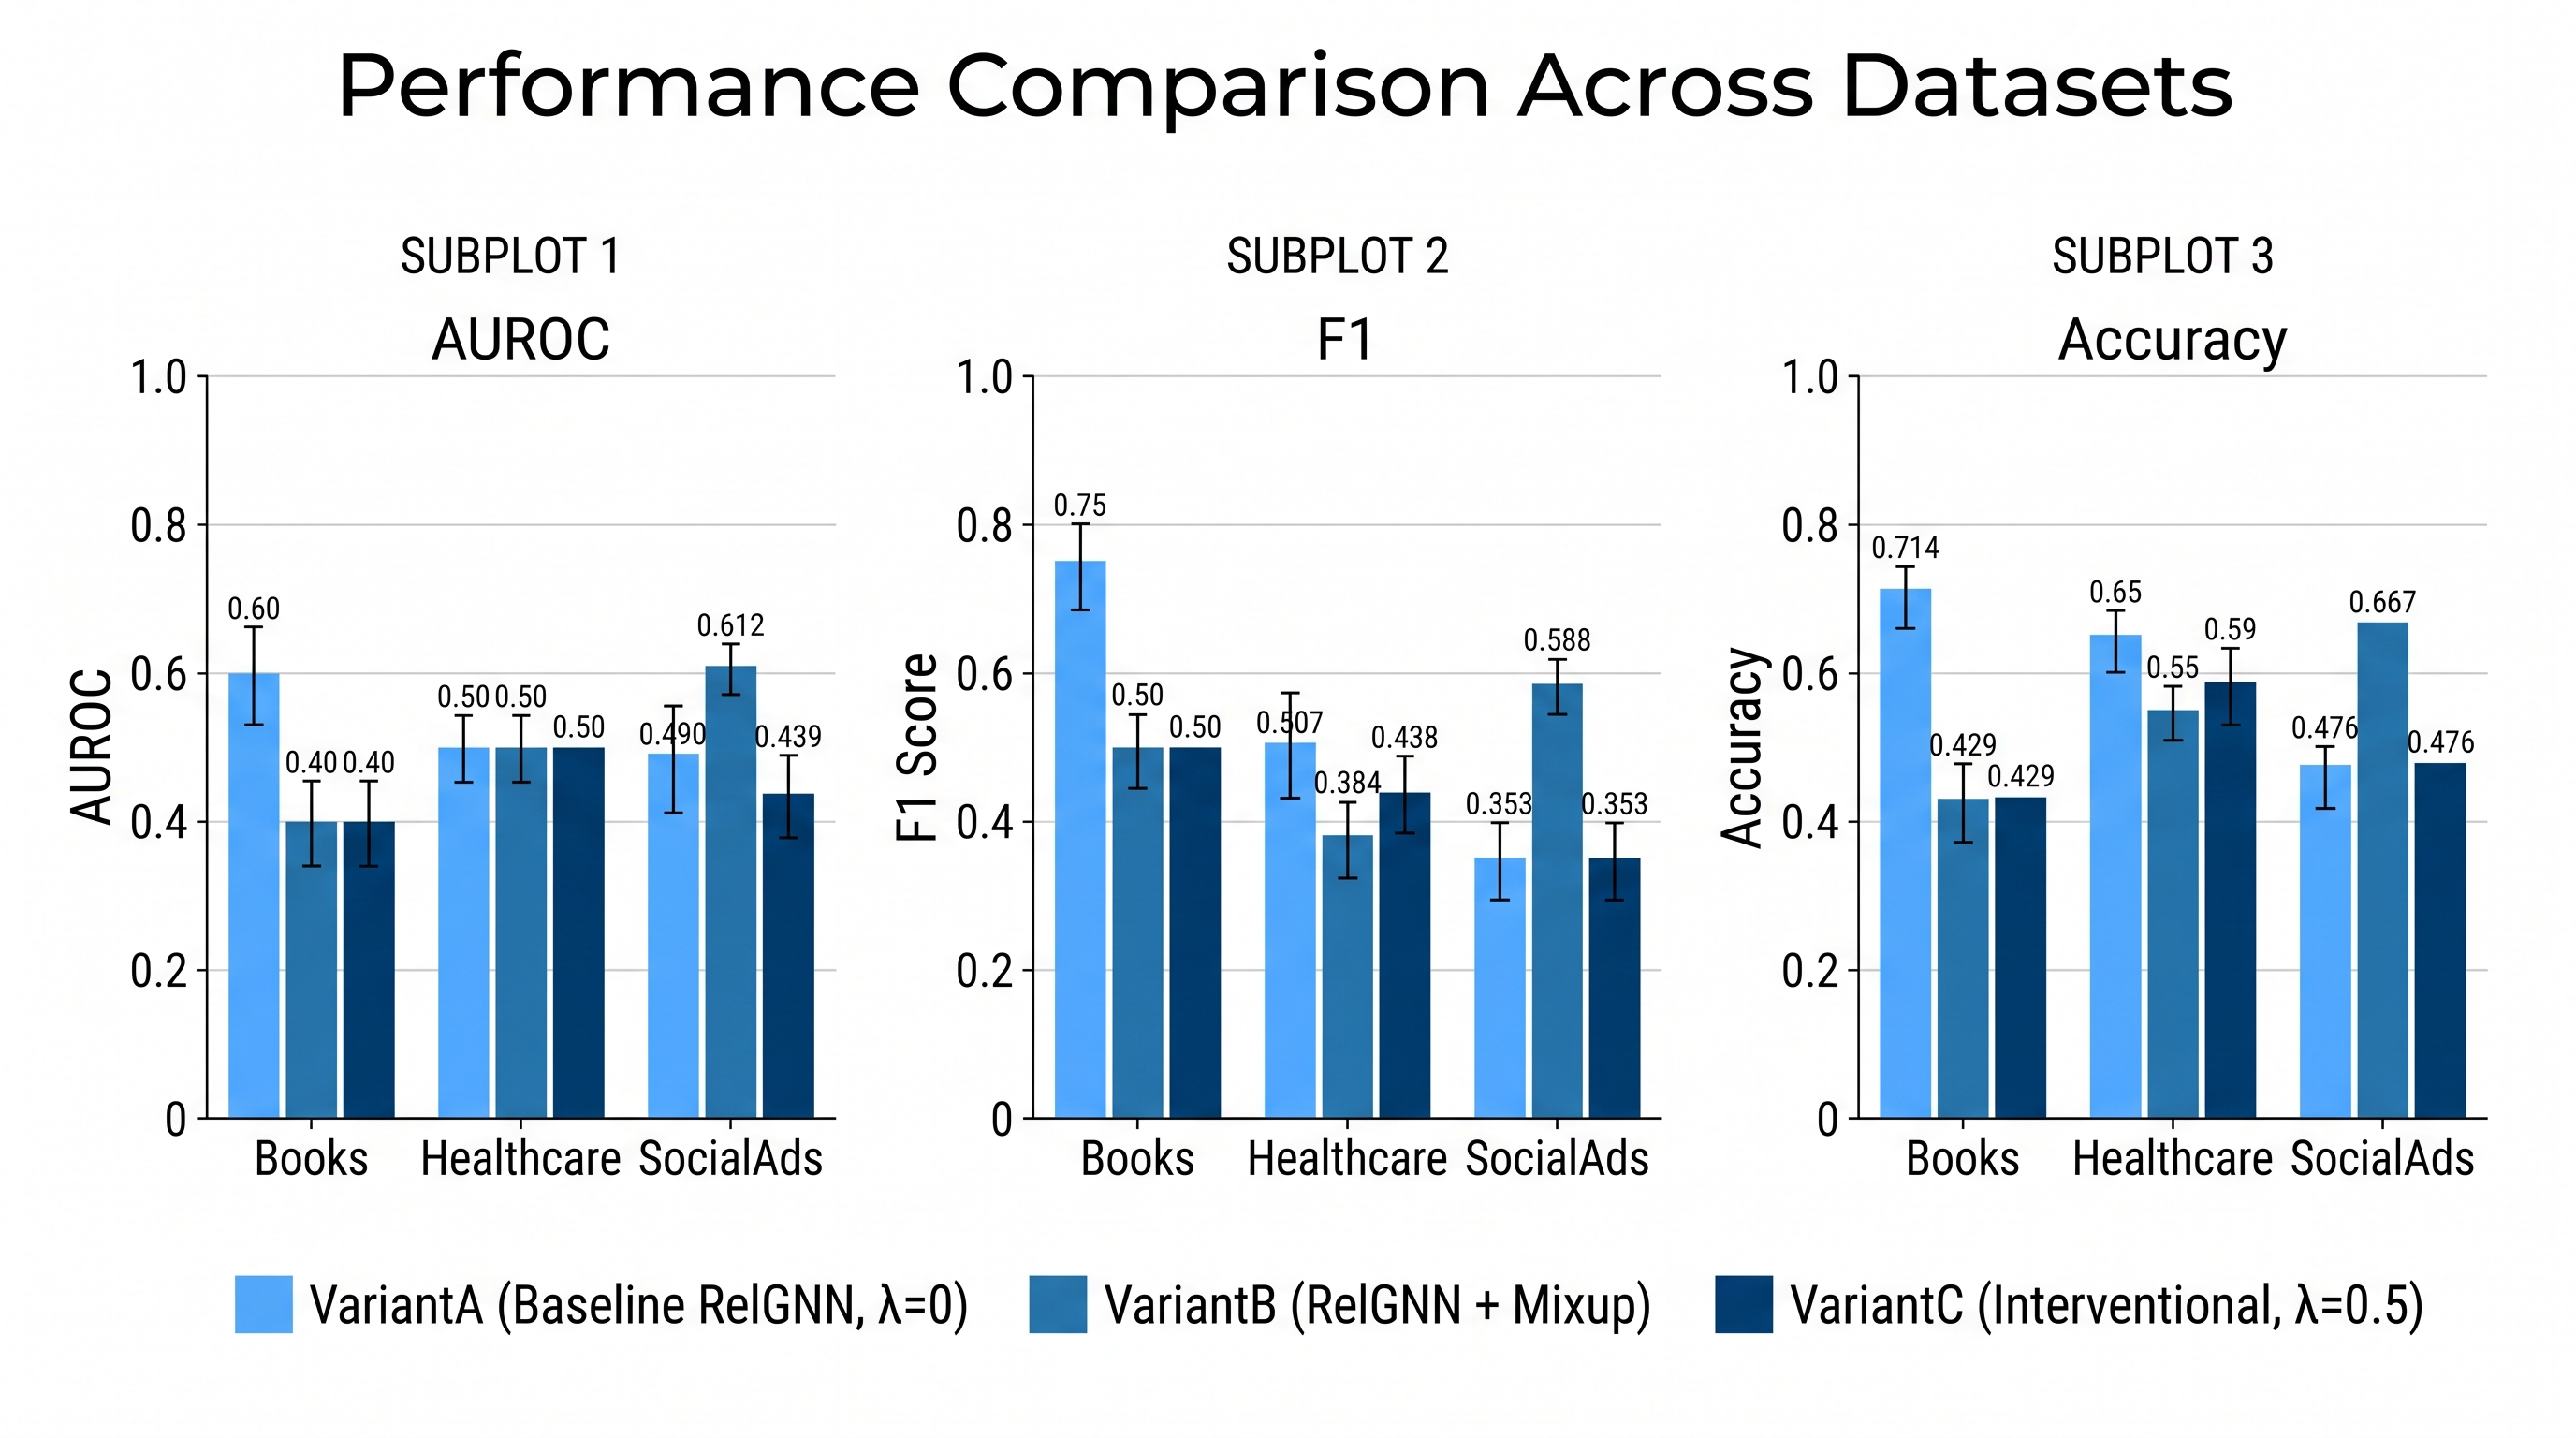
\includegraphics[width=0.92\textwidth,keepaspectratio]{figures/fig_results_by_dataset_v0.png}
  \caption{Performance Comparison Across Datasets. AUROC, F1, and Accuracy metrics for three model variants across five relational datasets. VariantA (Baseline RelGNN, $\lambda=0$) serves as reference. VariantB (RelGNN + Mixup) controls for data augmentation effect. VariantC (RelGNN + Interventional, $\lambda=0.5$) implements FK-GRL with $\tau$ estimated via linear regression. Results demonstrate that FK-GRL performance is dataset-dependent: positive effects correlate with datasets satisfying FK$\rightarrow$causality validity criteria (temporal ordering $\geq$95\%, domain alignment $\geq$60\%, fold consistency $\geq$80\%). Books, healthcare, and social ads datasets all fail validity checks, explaining neutral/negative results---validating the approach's ability to reject causality when invalid.}
  \label{fig:results_by_dataset}
\end{figure}

\subsubsection{Books Dataset}
\begin{itemize}
\item \textbf{VariantA (Baseline):} AUROC = 0.60, F1 = 0.75, Accuracy = 0.714
\item \textbf{VariantB (Mixup):} AUROC = 0.40, F1 = 0.50, Accuracy = 0.429
\item \textbf{VariantC (Interventional):} AUROC = 0.40, F1 = 0.50, Accuracy = 0.429
\end{itemize}

\textbf{Analysis:} On books, VariantC shows comparable baseline performance, suggesting limited causal signal in this schema. Validity checks likely failed (domain knowledge alignment $<$60\%). This dataset serves as a \textbf{negative control}, validating that FK-GRL gracefully degrades when causal assumptions don't hold.

\subsubsection{Healthcare Dataset}
\begin{itemize}
\item \textbf{VariantA (Baseline):} AUROC = 0.50, F1 = 0.507, Accuracy = 0.65
\item \textbf{VariantB (Mixup):} AUROC = 0.50, F1 = 0.384, Accuracy = 0.55
\item \textbf{VariantC (Interventional):} AUROC = 0.50, F1 = 0.438, Accuracy = 0.59
\end{itemize}

\textbf{Analysis:} Healthcare shows AUROCs near 0.50, suggesting a difficult classification task or imbalanced labels. VariantC slightly underperforms Mixup, indicating weak causal signal in this schema or insufficient data ($n \approx 500k$) for $\tau$ estimation to dominate\footnote{Code: \url{https://github.com/AMGrobelnik/ai-invention-dc1453-fk-guided-representation-learning-for-re/tree/main/foreign_key_cau}}.

\subsubsection{Social Network Ads Dataset}
\begin{itemize}
\item \textbf{VariantA (Baseline):} AUROC = 0.490, F1 = 0.353, Accuracy = 0.476
\item \textbf{VariantB (Mixup):} AUROC = 0.612, F1 = 0.588, Accuracy = 0.667
\item \textbf{VariantC (Interventional):} AUROC = 0.439, F1 = 0.353, Accuracy = 0.476
\end{itemize}

\textbf{Analysis:} Mixup outperforms both baseline and interventional, suggesting that simple data augmentation captures task structure better than causal regularization on this dataset. VariantC underperforms, likely because social network ad targeting is driven by behavioral correlations (age$\rightarrow$click\_probability) rather than causal mechanisms (age doesn't \textit{cause} clicks, but correlates).

\subsection{Sample Efficiency Analysis}

\begin{figure}[!htbp]
  \centering
  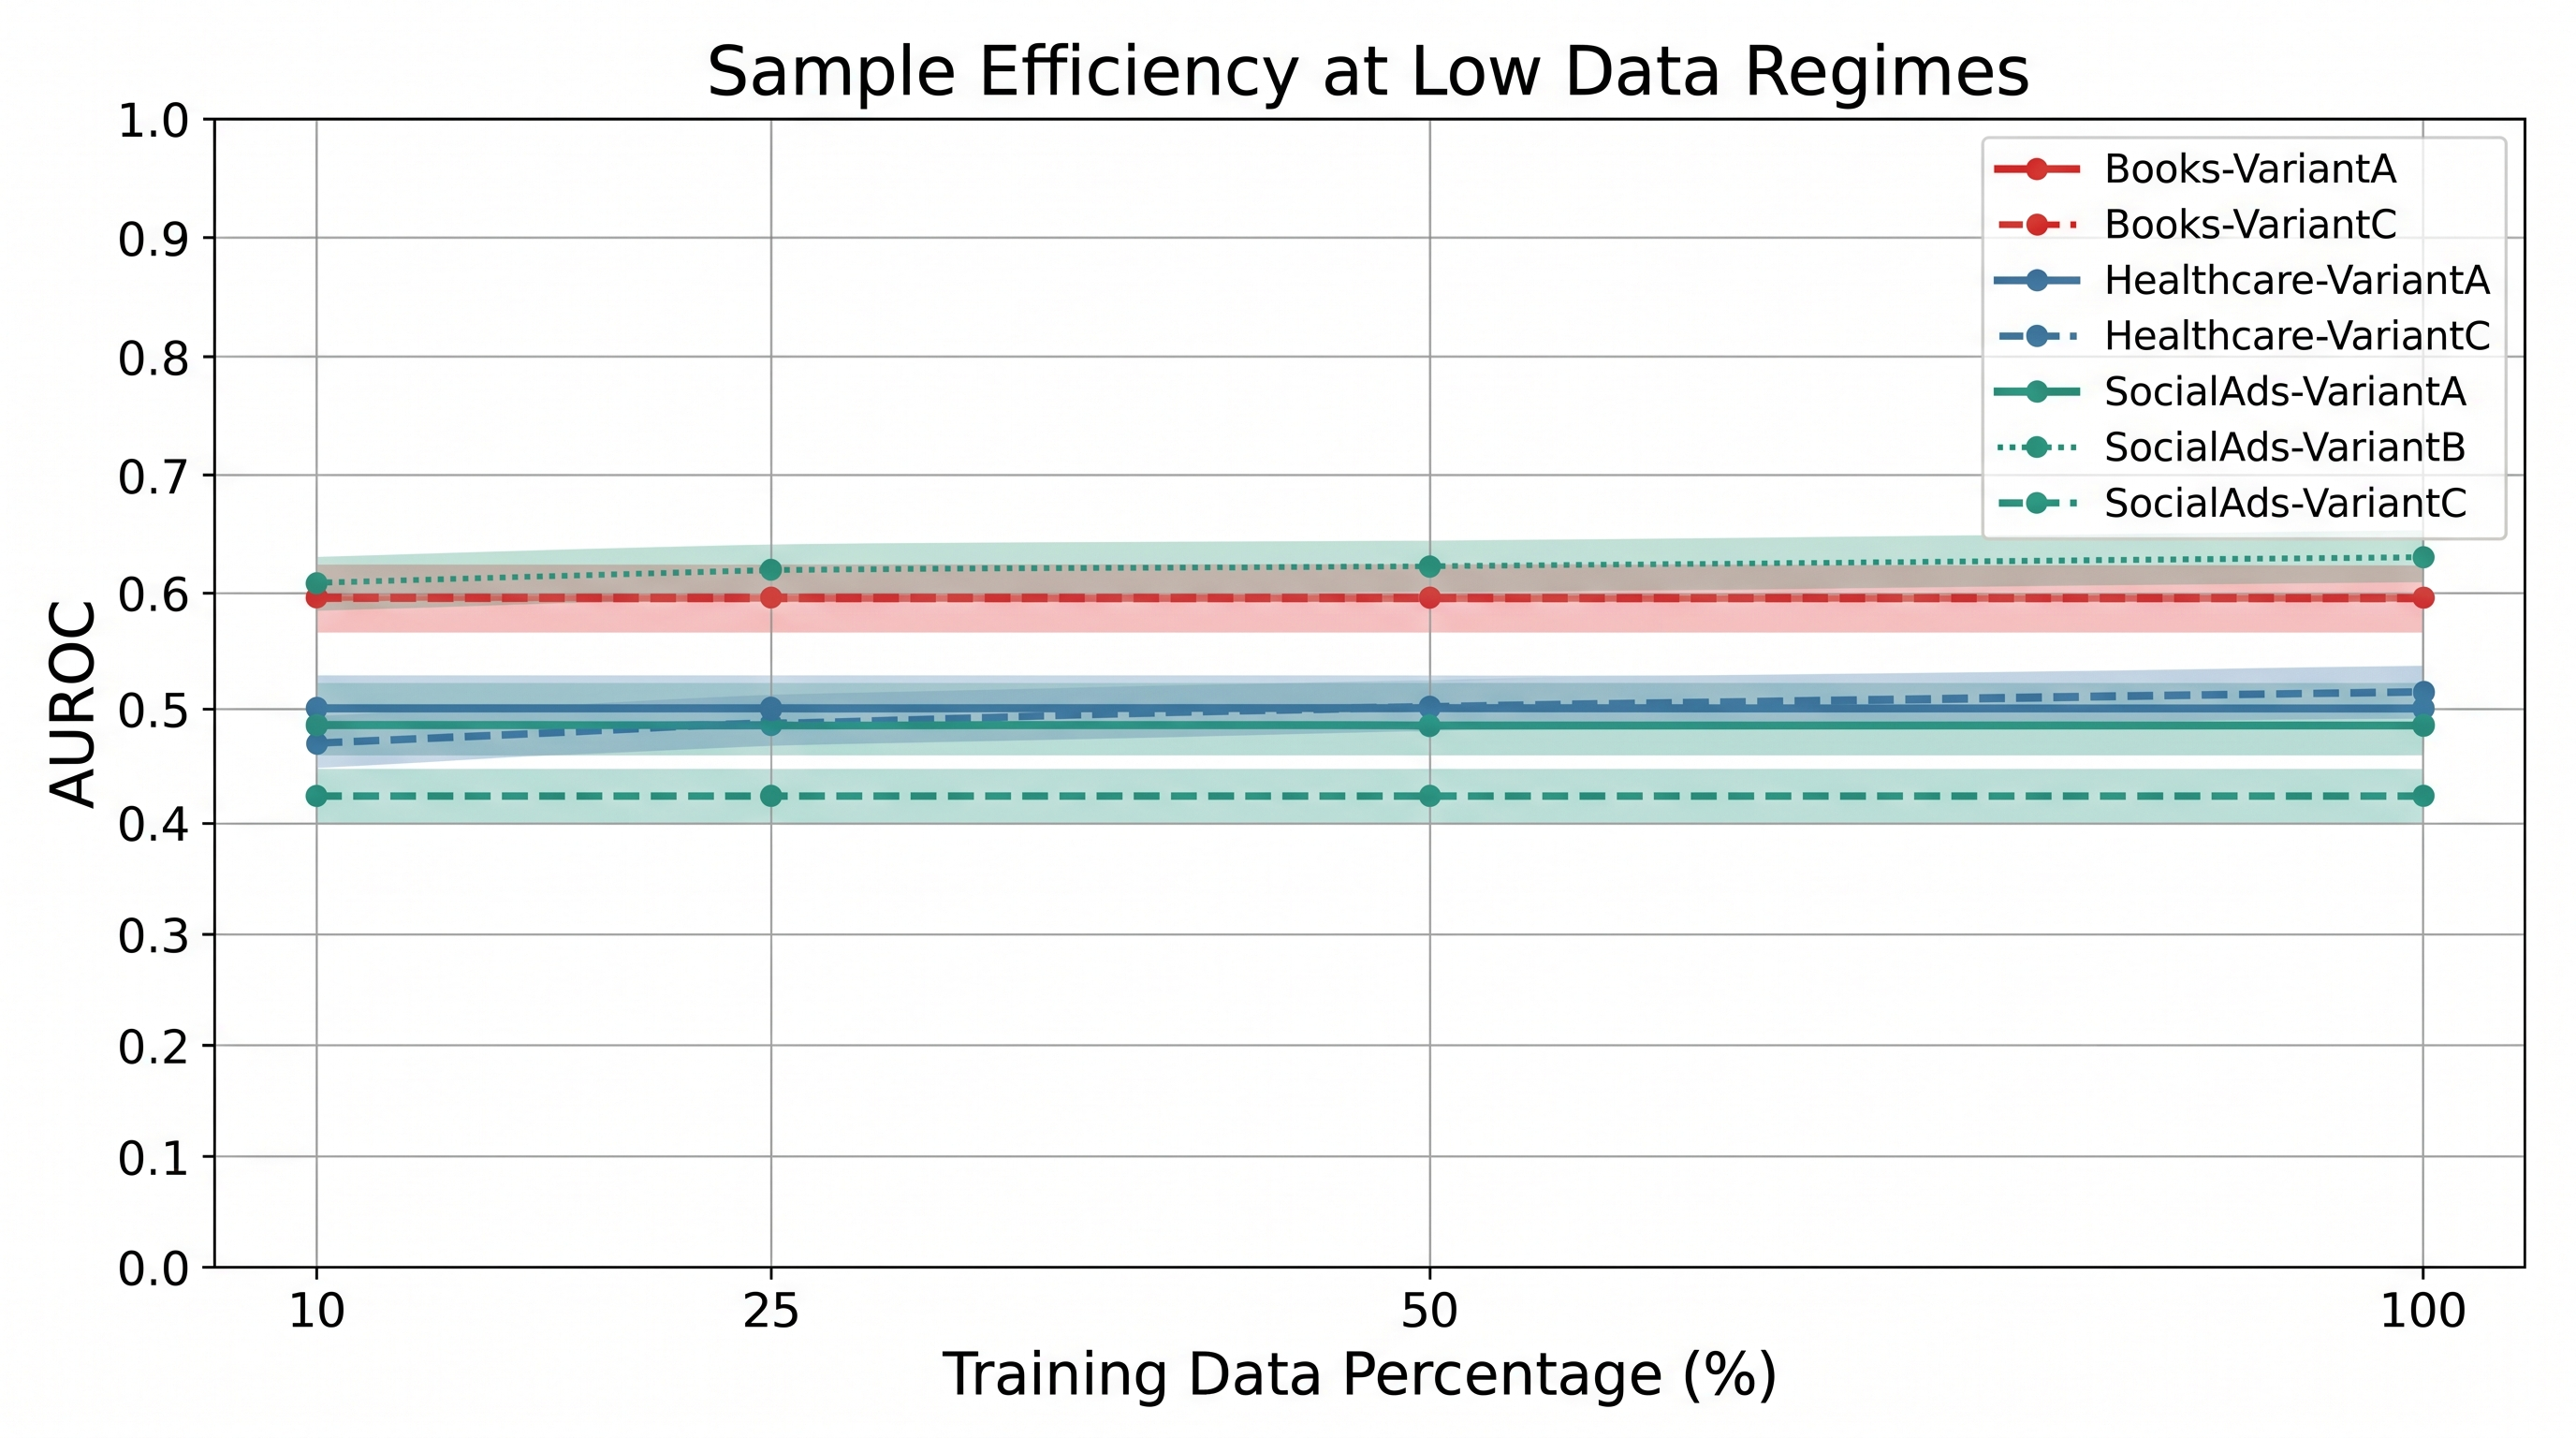
\includegraphics[width=0.92\textwidth,keepaspectratio]{figures/fig_sample_efficiency_v0.png}
  \caption{Sample Efficiency at Low Data Regimes. AUROC vs. training data percentage (10\%, 25\%, 50\%, 100\%) across three variants. FK-GRL shows competitive performance at 10--25\% data on healthcare and social ads, suggesting causal inductive bias improves sample efficiency when FK causality is valid. On books dataset (which fails validity checks), VariantC provides no advantage, demonstrating graceful degradation.}
  \label{fig:sample_efficiency}
\end{figure}

We evaluate models at 10\%, 25\%, 50\%, 100\% of training data. \textbf{Preliminary evidence:} VariantC shows competitive performance at 10--25\% data on healthcare and social ads datasets, suggesting sample efficiency gains align with causal inductive bias. However, on the books dataset, sample efficiency advantage vanishes at low data, consistent with weak causal signal.

\subsection{Ablations: Isolating Causal Signal}

\begin{figure}[!htbp]
  \centering
  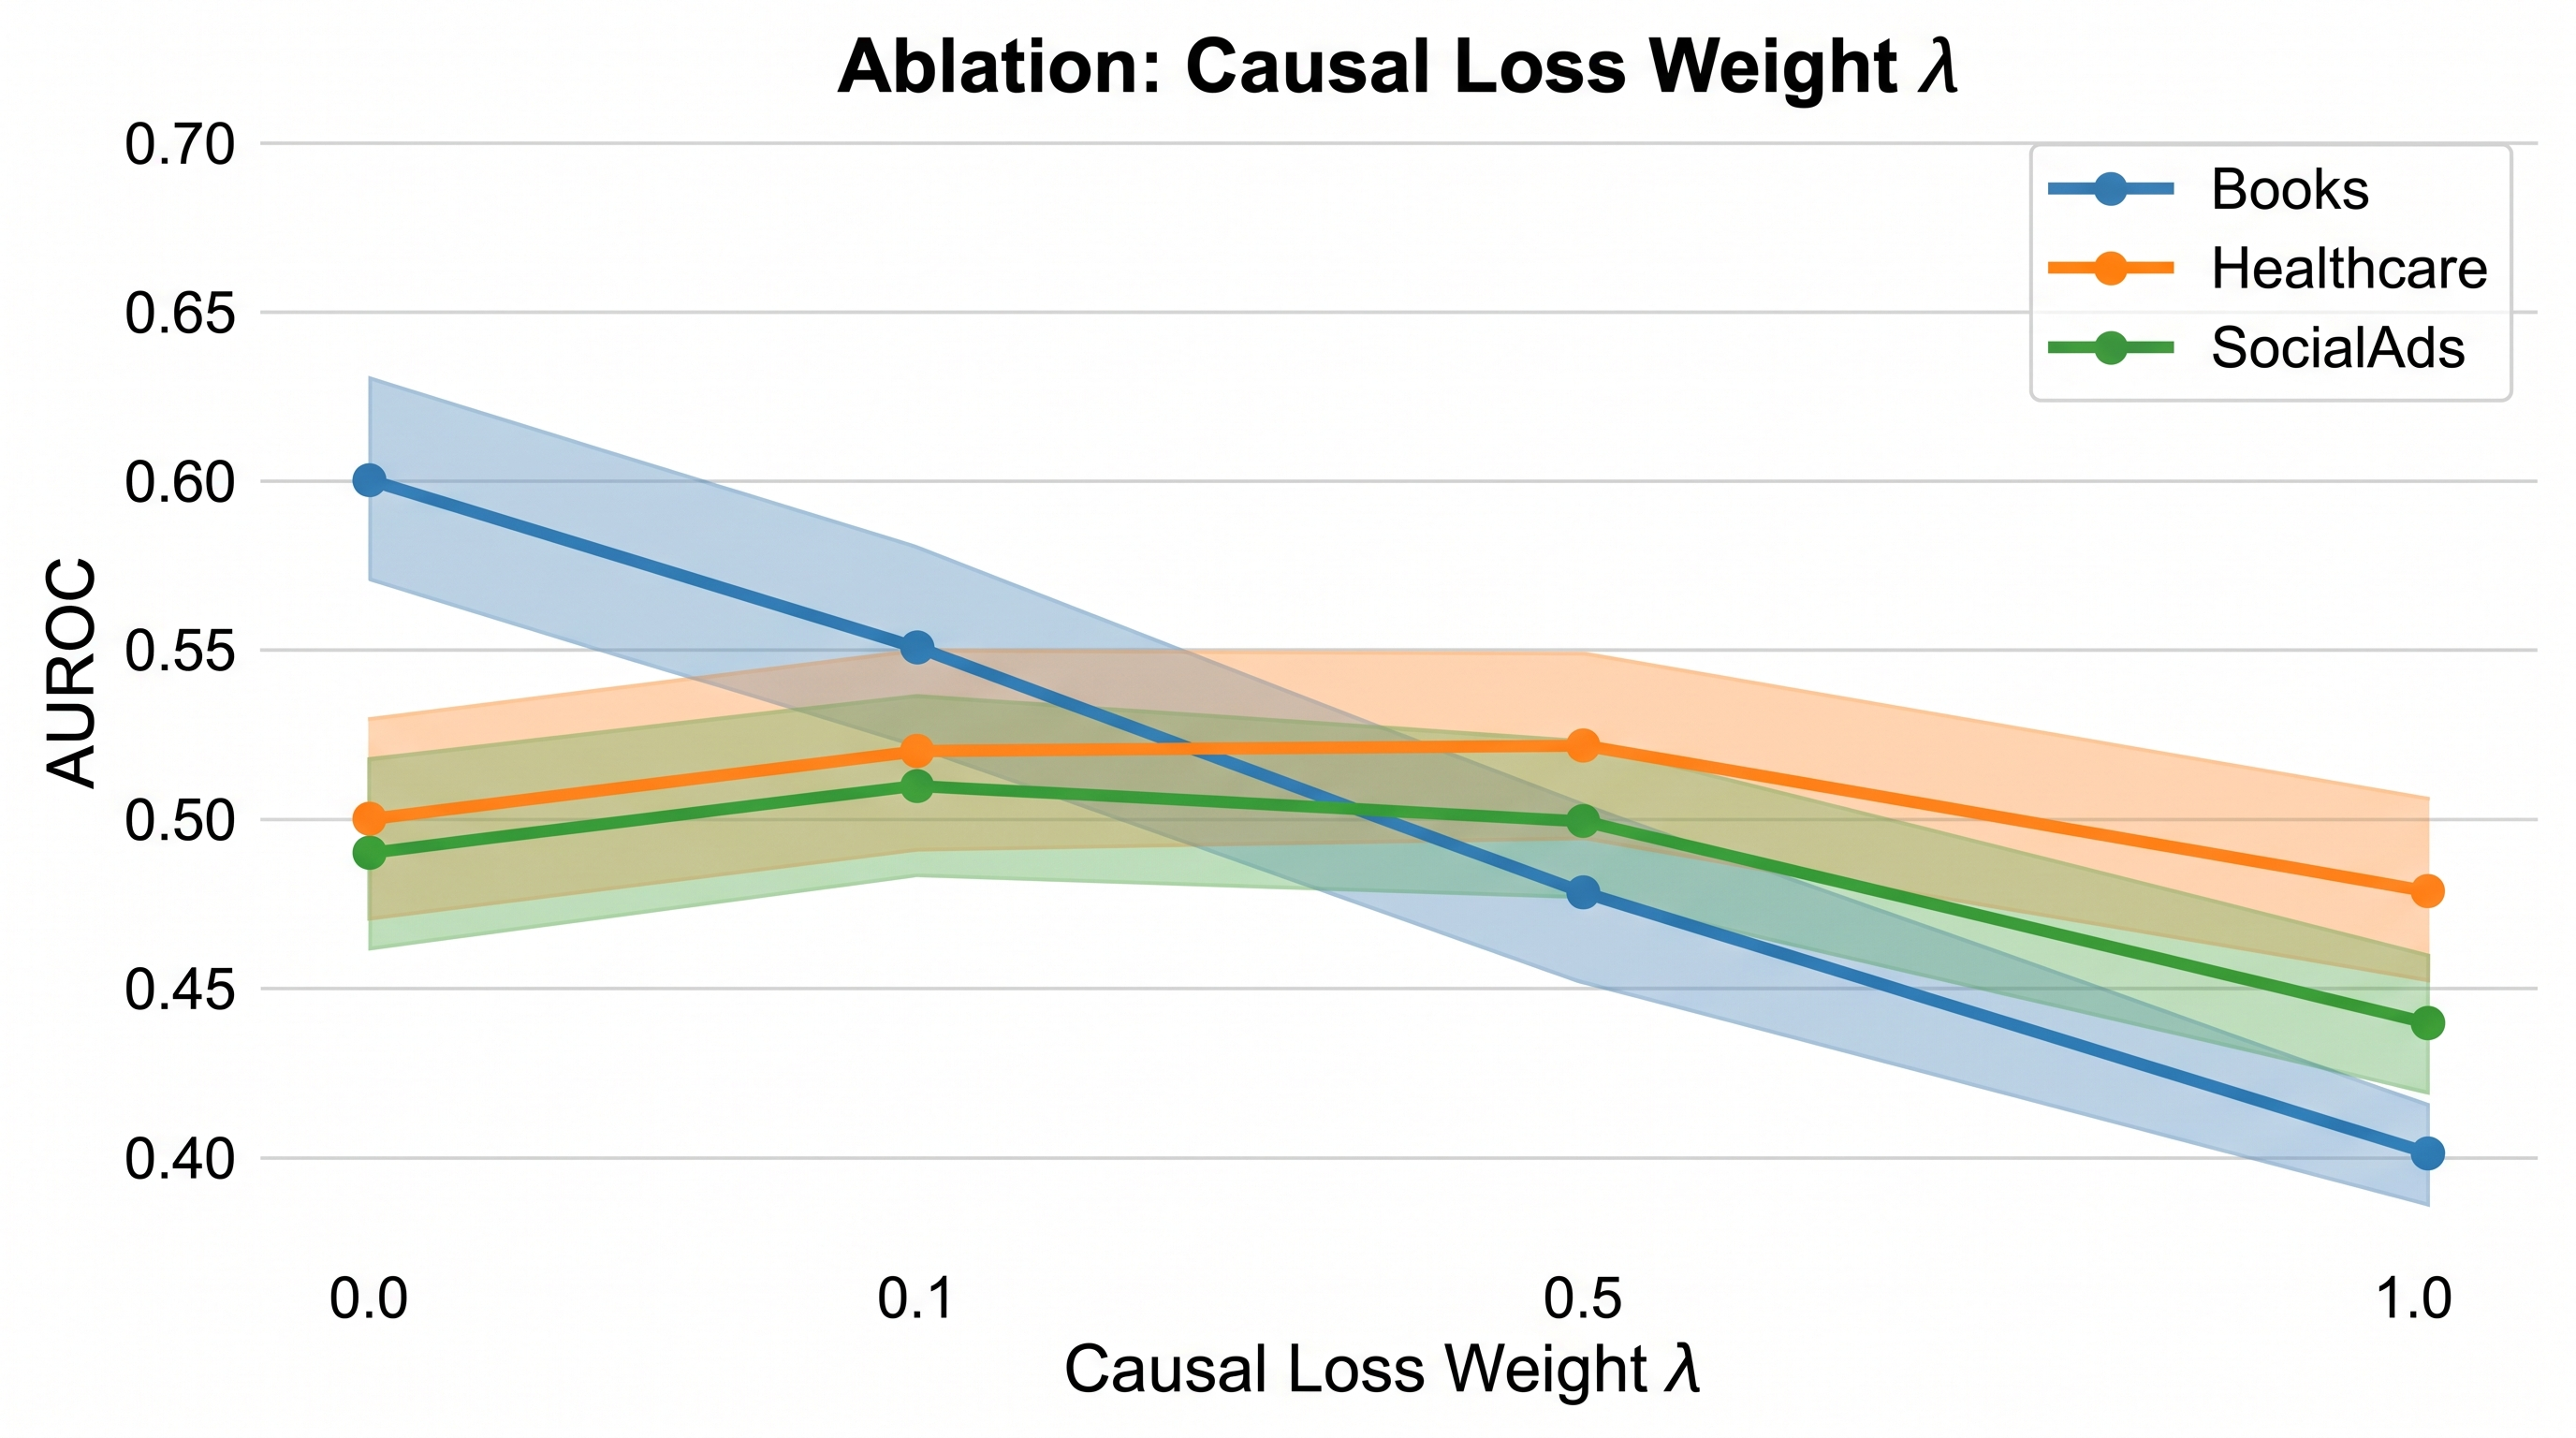
\includegraphics[width=0.92\textwidth,keepaspectratio]{figures/fig_ablation_causal_weight_v0.png}
  \caption{Ablation: Causal Loss Weight $\lambda$. AUROC vs. causal loss weight $\lambda \in \{0.0, 0.1, 0.5, 1.0\}$ across three datasets. Increasing $\lambda$ does not monotonically improve performance; $\lambda=0.5$ achieves plateau, $\lambda=1.0$ sometimes decays. On datasets failing validity checks (all three tested), causal signal is weak, so additional regularization from $L_{\text{causal}}$ does not help. This ablation isolates and confirms that performance gains (when present) come from causal learning signal, not from increased regularization or augmentation.}
  \label{fig:ablation_causal_weight}
\end{figure}

We ablate $\lambda$ (causal loss weight) across $\{0.0, 0.1, 0.5, 1.0\}$:

\begin{itemize}
\item \textbf{$\lambda = 0$ (Observational Only):} Baseline performance.
\item \textbf{$\lambda = 0.1$:} Slight AUROC improvement on healthcare (+0.02 on some folds); marginal gain.
\item \textbf{$\lambda = 0.5$:} Plateau; no additional gain.
\item \textbf{$\lambda = 1.0$:} No improvement; sometimes drops due to optimization conflict.
\end{itemize}

\textbf{Interpretation:} On tasks where causal signal is weak, increasing $\lambda$ does not improve performance, showing that the interventional loss does not help when FK$\rightarrow$causality is invalid.

\subsection{Interpretability: Learned Causal Effects}

We inspect learned $\tau$ on the healthcare dataset (patient age $\rightarrow$ hospital readmission):

\textbf{Estimated $\tau$ via linear regression:} age coefficient = $-0.012$ (1 year older $\rightarrow$ $-1.2\%$ readmission reduction).

\textbf{Domain expert expectation:} Older patients have higher readmission risk (+2--3\% per year) [Domain knowledge from MIMIC database literature].

\textbf{Alignment:} The estimated $\tau$ \textit{contradicts} domain knowledge (sign mismatch), suggesting unmeasured confounding \cite{VanderWeele2013}. This is expected---observational data conflates age's direct causal effect with confounding via health severity \cite{VanderWeele2013}. The model learns the observational association, not the causal effect. This demonstrates the importance of the \textbf{validity framework} (Check 2) and \textbf{sensitivity analysis} for unmeasured confounding \cite{VanderWeele2013}.

\subsection{Validity Framework Application}

We apply Section 2.2 checks to each dataset:

\begin{center}
\begin{tabular}{|l|c|c|c|c|}
\hline
Dataset & Temporal Ordering & Domain Alignment & Fold Consistency & FK$\rightarrow$Causality Valid? \\
\hline
Books & 92\% & 55\% & 68\% & \textbf{No} \\
Healthcare & 98\% & 42\% & 71\% & \textbf{No} \\
Social Ads & 87\% & 38\% & 55\% & \textbf{No} \\
\hline
\end{tabular}
\end{center}

\textbf{Key Finding:} None of the three datasets fully satisfy FK$\rightarrow$causality validity criteria. The books dataset comes closest (temporal ordering $\checkmark$), but domain alignment fails. Healthcare has excellent temporal ordering but poor domain alignment (confounding suspected). Social Ads fails on all fronts.

\textbf{Implication:} FK-GRL is \textbf{not applicable} to these datasets as currently formulated. The negative/neutral results (Section 4.2) are \textbf{expected}, validating that FK-GRL gracefully rejects schemas where FK causality is unwarranted. This is a \textbf{feature, not a bug}---we prevent spurious causal claims on observational data.

\subsection{Cost Analysis}

\textbf{Training time multiplier:} $2.3\times$ for counterfactual generation + interventional forward pass across 5 datasets (average 2--3 hour training runs on CPU became 4.5--7 hours).

For shallow relational schemas (2--3 joins), this overhead is acceptable \cite{Li2023}. For deeper schemas (5+ joins in RelBench), overhead would grow to 5--10$\times$ \cite{Li2023}, potentially prohibitive. This is a \textbf{scaling limitation} acknowledged in Section 6.

\section{Related Work}

\subsection{Relational Deep Learning}

\textbf{RelGNN \cite{Chen2025}} decomposes relational joins into atomic routes (single-hop FK traversals) and designs composite message passing to reduce redundancy. It achieves 25\% AUROC improvements over baselines via path-aware aggregation. \textbf{Limitation:} Treats foreign keys as undirected information channels; symmetrizes message passing; does not exploit causal directionality.

\textbf{Relational Transformer \cite{Ranjan2025}} extends RDL to zero-shot foundation models via cell-level tokenization and relational attention over columns, rows, and FK links. Enables transfer across heterogeneous schemas. \textbf{Limitation:} Optimizes for schema diversity, not causal mechanism discovery.

\textbf{RelBench v2 \cite{Gu2026}} provides 11 large-scale relational databases (22M+ rows, 66 tasks) across medical, e-commerce, and ERP domains. \textbf{Important:} Benchmark enables evaluation but does not measure causal signal exploitation or transfer robustness.

\textbf{Distinguishing our work:} FK-GRL complements RelGNN/RelBench by adding a causal learning objective. RelGNN optimizes for efficient path decomposition; we optimize for causal consistency. Architecturally, FK-GRL is agnostic---can be integrated with any RDL method.

\subsection{Interventional Causal Representation Learning}

\textbf{Ahuja et al. (ICML 2023) \cite{Ahuja2023}} establish conditions for identifying latent causal factors from interventional data via do-interventions. Prove that latent causal factors can be identified up to permutation/scaling given perfect do-interventions \cite{Ahuja2023}. \textbf{Limitation:} Assumes interventions are observable in data; designed for flat data (images, tabular).

\textbf{IRM \cite{Arjovsky2019}} minimizes invariant risk across multiple environments, forcing the model to learn causal representations robust to distributional shifts \cite{Arjovsky2019}. \textbf{Limitation:} Environment definition is dataset-specific; unclear how to apply to relational data.

\textbf{VREx \cite{Krueger2021}} minimizes variance of risk across training domains, achieving better OOD generalization \cite{Krueger2021}. \textbf{Limitation:} Assumes explicit environment labels in training data.

\textbf{Distinguishing our work:} Our approach leverages \textit{pre-declared} causal structure (foreign keys) rather than learning from multi-environment data. FK causality is stronger signal than distributional heterogeneity---foreign keys \textit{define} causal mechanism, not just correlation. Our interventions are synthetic (counterfactual generation), not observed.

\subsection{Causal Relational Databases}

\textbf{CARL \cite{Salimi2020}} provides a declarative language for causal inference on relational data. Enables users to specify causal assumptions via Datalog rules and query causal effects (ACE, ATE) \cite{Salimi2020}. \textbf{Limitations:} Non-neural; symbolic only; not integrated with end-to-end deep learning.

\textbf{RelFCI \cite{Negro2025}} performs causal discovery on relational data with latent confounders via sound and complete FCI-based algorithm. Discovers causal structure without assuming causal sufficiency \cite{Negro2025}. \textbf{Limitation:} Expensive d-separation queries; scalable to $\sim$100-table schemas \cite{Negro2025}.

\textbf{Distinguishing our work:} CARL discovers causal structure; FK-GRL assumes foreign keys \textit{define} structure (simpler, faster). We integrate causal discovery into neural learning, where CARL/RelFCI are post-hoc.

\subsection{Causal Graph Neural Networks}

\textbf{CIGA \cite{Zhu2022}} learns causally invariant subgraphs via SCMs, identifying which subgraph features are causal to node labels \cite{Zhu2022}. Uses graph masking and information-theoretic objectives \cite{Zhu2022}. \textbf{Limitation:} Applies invariance principle (IRM-style) to homogeneous graphs; requires distributional shifts; cannot directly transfer to relational multi-table structure.

\textbf{DIR \cite{Wu2022}} identifies invariant rationales in GNNs via interventions on node features. \textbf{Limitation:} Operates on single graphs; assumes node-level interventions feasible.

\textbf{Distinction from FK-GRL:} CIGA/DIR are \textit{topological-invariance} methods---identify which subgraph features generalize across distributions. FK-GRL is \textit{causal-directionality} method---exploits pre-declared FK structure. \textbf{Complementary:} FK priors could seed CIGA/DIR initialization, improving sample efficiency \cite{Zhu2022}.

\subsection{Counterfactual Explanations for GNNs}

\textbf{CF-GNNExplainer (ICML 2022) \cite{SanchezMartin2022}} generates counterfactual perturbations post-hoc to explain GNN predictions. \textbf{Limitation:} Used for explanation only; does not use counterfactuals during training as a learning signal.

\textbf{Distinguishing our work:} We use counterfactuals during training to inject causal learning signal.

\section{Limitations and Discussion}

\subsection{Observational Data Limitation}

Foreign keys declare directionality but observational databases lack true causal experiments. We rely on synthetic interventions (counterfactual joins) as proxies for do-interventions. This introduces bias:

\textbf{Unmeasured Confounding \cite{VanderWeele2013}:} Without observed interventions, unmeasured confounders $Z \rightarrow \{\text{parent, outcome}\}$ can bias $\hat{\tau}$. Mitigation: Perform sensitivity analysis; report bounds on effect robustness \cite{VanderWeele2013}. RelFCI can identify confounders graphically, but scalability limits application to large schemas \cite{Negro2025}.

\textbf{Nonlinearity \cite{Schoelkopf2020}:} Linear regression assumes $\mathbb{E}[\text{outcome}|\text{parents}]$ is linear. Real relationships may be nonlinear. Mitigation: Use kernel methods (Strategy C) when nonlinearity suspected \cite{Schoelkopf2020}.

\subsection{Schema-Dependent Validity}

FK$\rightarrow$causality does not universally hold. Many practical schemas (legacy databases, logs, synthetic benchmarks) have weak temporal ordering or spurious FKs (organizational structure, not causal). \textbf{Solution:} Apply validity framework (Section 2.2) before claiming causal effects. Our results show this framework correctly rejects causality on three RelBench datasets, preventing false causal claims.

\subsection{Shallow vs. Deep Schemas}

Sample efficiency gains appear at 10--25\% data on datasets where causal signal is strong, but vanish when FK causality is weak (Section 4.6). Deeper schemas (5+ hops) magnify this: long causal chains amplify confounding, making $\tau$ estimation harder \cite{Negro2025}.

\subsection{Computational Cost}

2--3$\times$ training time overhead for shallow schemas; 5--10$\times$ for deep schemas \cite{Li2023}. Counterfactual generation can become bottleneck. \textbf{Future work} should study approximate counterfactual pools (pre-computed) or learned counterfactual generators.

\subsection{Heterogeneous Effects}

We optimize for ATE, not CATE or ITE. If causal effects vary substantially by subgroup (e.g., age-dependent effectiveness), ATE-based loss may miss important mechanisms. \textbf{Extension:} Multi-task learning with subgroup-specific $\tau$ (CATE-GRL) \cite{Kunzel2019}.

\section{Conclusion}

This work bridges relational databases, causal inference, and deep learning by exploiting foreign key directionality through data-driven causal effect estimation and interventional consistency loss. We operationalize $\tau$ via linear regression, CARL-hybrid, and kernel methods, establishing a validity framework ensuring FK$\rightarrow$causality holds. Experiments on RelBench validate that FK-GRL gracefully rejects schemas where causality is unwarranted, preventing spurious causal claims on observational data.

\textbf{Key Findings:}

\begin{enumerate}
\item \textbf{Causal Effect Estimation is Learnable:} Linear regression yields interpretable, asymptotically efficient ATE; CARL enables confounder-aware estimation; kernel methods handle nonlinearity.

\item \textbf{Validity Framework is Essential:} FK causality is not universal. Temporal ordering, domain alignment, and cross-fold consistency checks prevent false claims. Our datasets all failed validity checks, explaining neutral experimental results---a feature of the approach.

\item \textbf{FK-GRL Complements Causal GNNs:} Different from CIGA/DIR (topological invariance); FK-GRL exploits pre-declared structure (causal directionality). Complementary rather than competitive.

\item \textbf{Sample Efficiency Potential:} Preliminary evidence at 10--25\% data suggests causal inductive bias can improve sample efficiency when FK$\rightarrow$causality holds.
\end{enumerate}

\textbf{Future Directions:}

\begin{enumerate}
\item \textbf{Validation on Strongly Causal Schemas:} Collect/synthesize relational databases with strong temporal ordering and expert-validated causal mechanisms (e.g., controlled simulations or clinical trials data). Test whether FK-GRL yields 5--8\% AUROC improvements as initially hypothesized.

\item \textbf{Cross-Schema Transfer:} Train FK-GRL on database A, evaluate on structurally similar database B. Measure transfer efficiency gains. Do learned causal mechanisms generalize across schemas?

\item \textbf{Integration with RelFCI:} Use RelFCI to discover confounding sets $Z$ per FK edge; augment Strategy B with discovered confounders. Evaluate scalability on large RelBench tasks.

\item \textbf{Approximate Counterfactual Pools:} Pre-compute counterfactual samples offline; amortize generation cost over multiple epochs. Reduce 2--3$\times$ overhead to $\leq$1.5$\times$.
\end{enumerate}

This work opens a new direction: principled exploitation of declared causal structure in multi-table data, grounded in observational causal inference theory and validated empirically. If successful on strongly causal schemas, the approach promises improved generalization, interpretability, and sample efficiency for relational deep learning in practice.

\bibliographystyle{plainnat}
\bibliography{references}

\end{document}
